\chapter{The Mechanical Way Of Living}

This chapter follows J. Krishnamurti's Brockwood Park dialogue on psychological security, mechanical order, fear, and time. The source material belongs to the Krishnamurti Foundation Trust corpus and is curated here by LazyingArt LLC through the Video2Book course project. There are no retained blackboard images or mathematical screenshots for this lecture, so the notation below is not a transcription of visible equations. It is a compact way of preserving the sequence of the inquiry: how the search for security becomes belief, how belief becomes image, how image requires occupation, and how occupation becomes a mechanical way of living.

\section{The Unfinished Question: Is Psychological Security Real?}

The dialogue begins by returning to a point left insufficiently clear the day before. The speakers had accepted that psychological security is a delusion, but the reason had not yet been shown. That matters because psychological security does not appear to most people as a luxury or error. It appears necessary. When a person is frightened, sorrowful, disturbed, or mentally unstable, he may feel that security must come first before any further inquiry is possible.

Krishnamurti's first move is therefore not to condemn the demand for security but to ask whether it exists at all. The form of the inquiry is simple:

\begin{equation}
\text{Is there psychological security?}
\end{equation}

The difficulty is that we begin by taking it for granted. We think we have it, or could get it, or would collapse without it. The conversation therefore has to slow down and ask what the word means. Psychological security is described as permanency, stability, and a well-founded sense of inner existence. It is what one can count on, hold to, be attached to, or trust not to perish.

A first schematic of the lecture's opening movement is:

\begin{equation}
\text{conditioning}
\longrightarrow
\text{search for psychological security}
\longrightarrow
\text{clinging}
\longrightarrow
\text{insecurity when disturbed}.
\end{equation}

This is not a psychological theory imposed on the dialogue. It is the conversation's own sequence. Conditioning gives importance to security; the person then clings to belief, knowledge, status, work, or relationship; and whatever is clung to becomes a source of anxiety because it can be disturbed.

\begin{table}
\centering
\begin{tabular}{|p{0.30\linewidth}|p{0.58\linewidth}|}
\hline
\textbf{Term} & \textbf{Working meaning in the dialogue} \\
\hline
Physical security & Bodily and material safety; necessary, but not the central issue under examination. \\
\hline
Psychological security & The inward demand for permanency, continuity, and something imperishable to depend on. \\
\hline
Belief & A projected support that gives comfort or a sense of continuity. \\
\hline
Image & A picture, symbol, or conclusion through which one sees oneself or another. \\
\hline
Conclusion & The psychological addition made by thought to actual facts. \\
\hline
Occupation & Not merely doing work, but being psychologically absorbed so that the brain feels ordered. \\
\hline
Mechanical order & Repetitive order that gives temporary safety but remains fragile and disturbed. \\
\hline
Actual perception & Direct seeing of what is so, distinguished from abstract agreement. \\
\hline
\end{tabular}
\caption{Transcript-grounded distinctions for the inquiry into security and mechanical living.}
\end{table}

\section{Belief, Knowledge, Status, And Permanency}

The conversation then gathers examples. A person may believe in heaven and feel that present trouble is temporary. Another may believe communism will finally solve everything. A scientist may feel secure in discovering permanent laws of nature. A doctor may feel secure in knowledge, position, patients, routine, status, and the continuity of work. A mother may find security in the child. Gold appears as an old symbol of the imperishable: something that does not corrode and can be counted on.

The examples are deliberately ordinary. The point is not that one belief is worse than another. The point is that each supplies a structure of dependence:

\begin{align}
\text{belief} + \text{continuity} &\longrightarrow \text{comfort}, \\
\text{knowledge} + \text{status} &\longrightarrow \text{felt permanence}, \\
\text{property} + \text{attachment} &\longrightarrow \text{``something to hold on to''}.
\end{align}

But the same structure contains conflict. If security depends on a profession, there may be illness, failure, age, war, depression, or social collapse. If it depends on a person, the relationship may alter. If it depends on belief, the belief must be defended. Thus the thing that promises stability becomes the thing that must be protected.

The first conclusion is modest but crucial: psychological security is not merely the possession of something. It is the inward movement of depending on something as though it could provide permanence.

\section{Security As Becoming In Time}

The inquiry then shifts from possession to time. One speaker says that security may be the anticipation that everything will be good in the future. If the present is lonely, painful, disappointing, or uncertain, thought projects a future in which the difficulty will be resolved. The future image then gives comfort now.

The schematic form is:

\begin{equation}
\text{present discomfort}
+
\text{anticipated future safety}
\longrightarrow
\text{felt security now}.
\end{equation}

This is the dialogue's first precise turn. Security becomes becoming. It is not only, ``I have something.'' It is also, ``I shall become something,'' or ``life will become better.'' The patient will find someone to love him. The ambitious person will become chief of the department. The professional will become famous. The religious person will reach heaven, reincarnation, or some permanent state. The structure is the same.

\begin{equation}
\text{psychological security}
\equiv
\text{becoming better in psychological time}.
\end{equation}

That equivalence must be handled carefully. It is not a formal theorem. It is a compact rendering of the lecture's movement: the demand for security has been uncovered as the demand that time should guarantee inward improvement.

\subsection{Question \& Answer}

\paragraph{Question.}
If there is no real psychological security, does that mean there is no psychological tomorrow? And if there is no psychological tomorrow, has all hope been taken away?

\paragraph{Answer.}
The lecture does not answer by offering a better hope. It clarifies what kind of tomorrow is being questioned. The ordinary tomorrow remains: practical time, appointments, work, physical arrangements, learning a skill. What is challenged is the psychological tomorrow in which the self becomes more secure, more permanent, more loved, more successful, more complete.

The difference can be written:

\begin{align}
\text{practical tomorrow} &: \text{necessary chronological arrangement}, \\
\text{psychological tomorrow} &: \text{projected becoming of the self}.
\end{align}

The dialogue's pressure falls on the second line. If security means the certainty that the self will become safe in time, then Krishnamurti asks whether such security exists at all.

\section{Idea, Fact, And Perception}

At this point the conversation refuses to rest with a general statement. One can agree that everything changes, that death comes, that money, health, relationship, and feeling cannot be counted on. But Krishnamurti calls this empirical argument superficial. The deeper question is why the fact does not act as a fact.

A person may hear, ``there is no psychological security,'' and make it into an idea. He may accept it abstractly and still continue in the old movement. That distinction becomes one of the lecture's central operators:

\begin{equation}
\text{idea} \not\Rightarrow \text{action},
\qquad
\text{perception} \Rightarrow \text{action}.
\end{equation}

The word ``operator'' should not mislead us. Nothing technical is being imported. The point is simply that an idea can be correct and still leave the structure intact. Perception is different. If there is direct seeing that one is clinging to something for security, then action is not added afterward as a method. In the dialogue's language, action comes through perception, not through ideation.

\subsection{Question \& Answer}

\paragraph{Question.}
Why does ``there is no security'' become an idea instead of an actual fact, like a table, a hand, or a flower?

\paragraph{Answer.}
Because the self that seeks security appears to itself as real. If the self is taken as an actual center, then it must protect itself. The statement that there is no security threatens that center. So thought translates the statement into an idea. As an idea it can be discussed, accepted, admired, or resisted without ending the movement of seeking security.

The lecture's working distinction is:

\begin{align}
\text{abstract assent} &: \text{``I understand there is no security''}, \\
\text{actual perception} &: \text{seeing the clinging as it operates}.
\end{align}

The first can continue indefinitely. The second changes the field in which the question is being asked.

\section{The Image Becomes More Real Than Reality}

The middle of the dialogue turns from security to image. If security lies in belief, profession, relationship, symbol, or conclusion, then one sees the world through that structure. The wife, the patient, the colleague, the profession, the house, and the belief all become arranged around the function they serve for the self.

Krishnamurti states the point sharply: the picture, the image, the conclusion is the security. The other speakers then ask why this image becomes so fantastically real, more real than the hills or the marble in front of them. This is the emotional and structural force of psychological security: the image feels solid even when the argument against it is clear.

The doctor example gives the cleanest analysis. We can write the identity as a sum, but only as a note-making device:

\begin{equation}
\text{doctor identity}
=
\text{training}
+
\text{knowledge}
+
\text{daily operation}
+
\text{psychological conclusion}.
\end{equation}

The first three terms are actual. Training took place. Knowledge has been acquired. Daily work is done. The last term is different. It includes comparison, status, continuity, fear of loneliness, and the feeling that without this role things would be bad.

\begin{table}
\centering
\begin{tabular}{|p{0.42\linewidth}|p{0.42\linewidth}|}
\hline
\textbf{Actual in the doctor example} & \textbf{Added by psychological conclusion} \\
\hline
Training & ``I am better than another'' \\
\hline
Knowledge & Status and professional self-image \\
\hline
Daily operation & Protection from loneliness \\
\hline
Seeing patients & Fear that without this role there is no activity \\
\hline
Functional skill & Continuity of identity as ``me'' \\
\hline
\end{tabular}
\caption{The doctor example separates actual function from the psychological surplus of identity.}
\end{table}

A useful derivation of the example is:

\begin{enumerate}
\item A person has training, knowledge, and daily activity.
\item Thought gathers those facts into the conclusion, ``I am this.''
\item The conclusion becomes a source of status, continuity, and protection.
\item The person then acts to maintain the conclusion.
\item The conclusion requires occupation, because without occupation loneliness and fear return.
\end{enumerate}

This is why the example leads directly into the title of the lecture. The self-image must be kept going. It needs a process. It needs occupation.

\section{Occupation, Mechanical Order, And Disorder Masked As Order}

The practical hinge of the dialogue is occupation. Occupation means more than activity. A person may be seeing patients, doing arithmetic, writing books, going to the laboratory, managing the house, joining a community, or pursuing entertainment. The psychological point is that the brain feels steadier when it is occupied.

The encephalograph anecdote is used only as a spoken illustration. A disturbed woman is said to show a wild pattern until she is occupied with arithmetic; then the pattern becomes smooth; when she stops, it goes wild again. We should not reconstruct an EEG graph from this, because no visual trace is available. But the conceptual sequence is clear:

\begin{equation}
\text{unoccupied brain}
\longrightarrow
\text{instability or fear}
\longrightarrow
\text{occupation}
\longrightarrow
\text{mechanical order}.
\end{equation}

The order is mechanical because it depends on the continuation of the occupation. It works for a little while. Then it becomes repetitive, boring, dull, or disturbed. The person moves to another process. The result is not freedom from disorder but disorder covered by repetition.

\begin{equation}
\text{mechanical order}
=
\text{disorder masked as order}.
\end{equation}

\begin{figure}
\centering
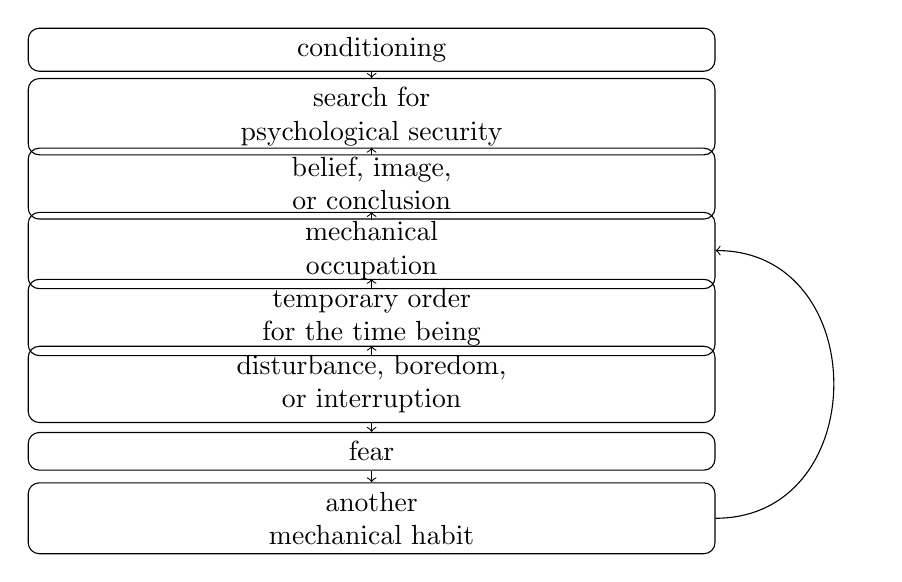
\begin{tikzpicture}[node distance=0.85cm]
\node[draw, rounded corners, align=center, text width=0.70\linewidth] (a) {conditioning};
\node[draw, rounded corners, align=center, text width=0.70\linewidth, below of=a] (b) {search for\\psychological security};
\node[draw, rounded corners, align=center, text width=0.70\linewidth, below of=b] (c) {belief, image,\\or conclusion};
\node[draw, rounded corners, align=center, text width=0.70\linewidth, below of=c] (d) {mechanical\\occupation};
\node[draw, rounded corners, align=center, text width=0.70\linewidth, below of=d] (e) {temporary order\\for the time being};
\node[draw, rounded corners, align=center, text width=0.70\linewidth, below of=e] (f) {disturbance, boredom,\\or interruption};
\node[draw, rounded corners, align=center, text width=0.70\linewidth, below of=f] (g) {fear};
\node[draw, rounded corners, align=center, text width=0.70\linewidth, below of=g] (h) {another\\mechanical habit};
\draw[->] (a) -- (b);
\draw[->] (b) -- (c);
\draw[->] (c) -- (d);
\draw[->] (d) -- (e);
\draw[->] (e) -- (f);
\draw[->] (f) -- (g);
\draw[->] (g) -- (h);
\draw[->] (h.east) .. controls +(2.0,0.0) and +(2.0,0.0) .. (d.east);
\end{tikzpicture}
\caption{A transcript-grounded reconstruction of the loop of mechanical security. This is an explanatory diagram, not a copied board figure.}
\end{figure}

\subsection{Question \& Answer}

\paragraph{Question.}
Why does the brain seem to go wild when it is not occupied, and why does mechanical order fail to be real order?

\paragraph{Answer.}
The dialogue says that in occupation there is security because there is order. But the order is only mechanical. It depends on content, repetition, and continuity. When the content stops, the instability returns. If the person becomes bored, he seeks something more interesting. If the mechanism is threatened, he becomes afraid. If one habit fails, he establishes another.

The process can be written as an update rule:

\begin{equation}
M_{n+1}
=
\begin{cases}
M_n, & \text{if the mechanism still gives temporary order},\\
\text{new habit}, & \text{if boredom, disturbance, or fear appears}.
\end{cases}
\end{equation}

Here \(M_n\) is only a notation for the current mechanical process. It is not a psychological model. It records the lecture's repeated movement: one mechanical process is replaced by another, and this replacement is called living.

\section{Why The Brain Remains Mechanical}

The later dialogue asks a sharper question: why does the brain become mechanical, and why does it remain mechanical? The first answers are partial. Mechanical life is repetitious. It is action and reaction. It is easy. It gives boundaries. It feels safe. But Krishnamurti presses further.

The brain wants order. Without order it cannot function properly. Since mechanical order appears safe for the time being, the brain accepts it and hopes it will not lead to disaster. This is the trap. It is not simply that mechanical living is chosen once. A structure is built around it, and then the fear of losing that structure keeps it going.

\begin{align}
\text{brain needs order}
&\longrightarrow
\text{accepts mechanical process}, \\
\text{mechanical process disturbed}
&\longrightarrow
\text{fear of collapse}, \\
\text{fear of collapse}
&\longrightarrow
\text{renewed mechanical process}.
\end{align}

Conditioning reinforces the pattern. Tradition, education, culture, childhood obedience, communities, professional reputation, and collective belief all train the brain to find order mechanically. Even the attempt to leave one mechanism may become another mechanism. One leaves a profession, a belief, or a domestic routine, and joins a community, a movement, or another repetitive form.

The lecture then states the central late proposition.

\begin{proposition}
The mechanical way of living leads to disorder, even though it is adopted in the hope of order.
\end{proposition}

\begin{proof}
The proof here is not formal deduction but the ordered argument of the dialogue.
\begin{enumerate}
\item The brain needs order in order to function.
\item It accepts a mechanical process because that process gives order for the time being.
\item The process depends on repetition, continuity, and external or internal conditions.
\item Life disturbs those conditions.
\item When disturbance appears, fear appears.
\item To escape fear, the brain establishes another mechanical habit.
\item Therefore the original order was not total order; it was disorder maintained under the appearance of order.
\end{enumerate}
\end{proof}

At this point Krishnamurti speaks of instant action and an order that is not fragmented. The dialogue must preserve the tension here. One participant immediately objects that this does not yet follow logically. Krishnamurti does not dismiss the objection. He says they can go into it only if the mechanical security developed, attached to, and cultivated by the brain is actually perceived.

\section{When The Past Meets The Present}

The closing movement brings the whole inquiry into time and relationship. The speakers turn from mechanical habit to the past. We meet another person through memories, images, reputation, words, pictures, and symbols. With that past, we meet the person now. Therefore, in the dialogue's phrase, the past meets the present.

A compact notation for this is:

\begin{equation}
\text{past}
=
\{\text{memory},\text{image},\text{reputation},\text{word},\text{picture},\text{symbol}\}.
\end{equation}

If this past continues through the present, relationship is no longer direct. One is meeting an image, not the person. The person may have changed, but the old memory continues. Krishnamurti calls this one of the factors of time movement, bondage, fear, and disorder.

\begin{equation}
\text{past meets present and continues}
\longrightarrow
\text{time movement}+\text{bondage}+\text{fear}.
\end{equation}

The alternative is not a method for suppressing memory. The dialogue does not say, ``make the past stop.'' It asks whether the movement can be completely observed as it happens. If it is completely observed, Krishnamurti says, it stops. Then one meets the other freshly.

\begin{equation}
\text{complete awareness of the movement}
\longrightarrow
\text{the movement stops}.
\end{equation}

\begin{figure}
\centering
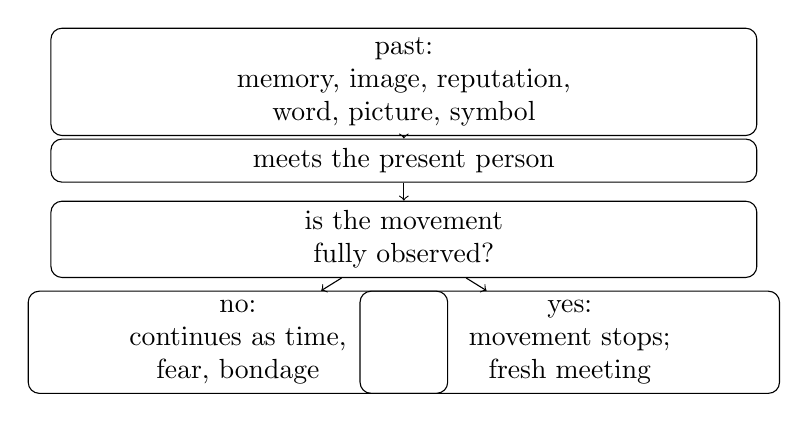
\begin{tikzpicture}[node distance=1.0cm]
\node[draw, rounded corners, align=center, text width=0.72\linewidth] (past) {past:\\memory, image, reputation,\\word, picture, symbol};
\node[draw, rounded corners, align=center, text width=0.72\linewidth, below of=past] (present) {meets the present person};
\node[draw, rounded corners, align=center, text width=0.72\linewidth, below of=present] (choice) {is the movement\\fully observed?};
\node[draw, rounded corners, align=center, text width=0.42\linewidth, below left of=choice, xshift=-1.4cm, yshift=-0.6cm] (cont) {no:\\continues as time,\\fear, bondage};
\node[draw, rounded corners, align=center, text width=0.42\linewidth, below right of=choice, xshift=1.4cm, yshift=-0.6cm] (stop) {yes:\\movement stops;\\fresh meeting};
\draw[->] (past) -- (present);
\draw[->] (present) -- (choice);
\draw[->] (choice) -- (cont);
\draw[->] (choice) -- (stop);
\end{tikzpicture}
\caption{The final relationship structure: the past meets the present, and the question is whether that movement continues.}
\end{figure}

The chapter should not make this ending sound complete. The dialogue itself does not. Near the close, Krishnamurti says they have not really tackled the root of all this: the disturbance, turmoil, travail, anxiety, and wild disorder of the brain. The last question remains open: why do human beings live this way? The final answer named in the dialogue is brief and double-edged: time.

\section{Summary}

The lecture begins with psychological security and ends with time. Between those two points it traces a disciplined path: security is first seen as belief, status, knowledge, property, and relationship; then as becoming in the future; then as an idea that has not become fact; then as image and conclusion; then as occupation; then as mechanical order; then as the continuation of the past into the present.

The mathematical forms in this chapter are only schematics. Their value is to keep the order of the inquiry visible. The central chain is:

\begin{equation}
\text{security}
\longrightarrow
\text{image}
\longrightarrow
\text{occupation}
\longrightarrow
\text{mechanical order}
\longrightarrow
\text{disorder}
\longrightarrow
\text{time}.
\end{equation}

What remains unresolved is not a minor detail but the next fundamental inquiry: why the brain lives in this disturbance at all, and whether seeing the whole movement is already the beginning of a different order.